% AER-Article.tex for AEA last revised 22 June 2011
\documentclass[AER]{AEA}

% The mathtime package uses a Times font instead of Computer Modern.
% Uncomment the line below if you wish to use the mathtime package:
%\usepackage[cmbold]{mathtime}
% Note that miktex, by default, configures the mathtime package to use commercial fonts
% which you may not have. If you would like to use mathtime but you are seeing error
% messages about missing fonts (mtex.pfb, mtsy.pfb, or rmtmi.pfb) then please see
% the technical support document at http://www.aeaweb.org/templates/technical_support.pdf
% for instructions on fixing this problem.

% Note: you may use either harvard or natbib (but not both) to provide a wider
% variety of citation commands than latex supports natively. See below.

% Uncomment the next line to use the natbib package with bibtex 
\usepackage{natbib}

%%%%%% Added packages and declarations
\RequirePackage{amsfonts,amsmath,graphicx,booktabs}

% Uncomment the next line to use the harvard package with bibtex
%\usepackage[abbr]{harvard}

% This command determines the leading (vertical space between lines) in draft mode
% with 1.5 corresponding to "double" spacing.
\draftSpacing{1.5}
\newlength\TableWidth
\usepackage{array}
\newcolumntype{H}{>{\setbox0=\hbox\bgroup}c<{\egroup}@{}}

\begin{document}

\title{Should Anyone Pay Attention to Euler?}
\shortTitle{Should Anyone Pay Attention to Euler?}
\author{Edmund Crawley\thanks{ Federal Reserve Board, 20th Street and Constitution Avenue N.W., Washington, DC 20551, edmund.s.crawley@frb.gov. The analysis and conclusions set forth are those of the author alone and do not indicate concurrence by other members of the research staff or the Board of Governors.}}
\date{\today}
\pubMonth{}
\pubYear{}
\pubVolume{}
\pubIssue{}
\JEL{}
\Keywords{Rational Inattention, Euler, Monetary Policy}

\begin{abstract}

\end{abstract}


\maketitle

\newpage
\section{Introduction}
Basic idea
\begin{itemize}
\item Losses from inattention to interest rates for consumption smoothers (with no refinance decision) are second order
\item Losses from inattention to interest rates for constrained agents are first order
\item Losses from inattention to interest rates for refinance decisions are first order
\item What happens if only the constrained/refinancing agents pay attention?
\end{itemize}

Relation to literature
\begin{itemize}
\item \cite{wong_population_2016}, \cite{berger_prepayment_2018}, \cite{eichenbaum_refinance_2018}. These papers use a exogenous real interest rate (small open economy) to show that `monetary policy' works to a large degree through this mortgage and refinancing channel. In these models the long term real interest rate is what matters.
\item \cite{greenwald_mortgage_2018}, \cite{garriga_monk_2019}. These papers show how mortgages affect the transmission mechanism in a New Keynesian closed economy setting. In contrast to the small open economy papers, these run into the problem that the central bank has no power over the long term real interest rate, and therefore the mechanisms do not carry through. They find mortgages can affect transmission, but only in the case where the inflation target is changed.
\item The inattention by unconstrained agents in this paper should marry these two strands of the literature. We hopefully can get the results from the small open economy models passing through to a New Keynesian settings, where the central bank has power over long rates because unconstrained consumers are not paying attention to these rates.
\end{itemize}
Evidence of inattention:
\begin{itemize}
\item Historical evidence on consumers not following Euler (Hall?)
\item Cross-sectional evidence - what is it? Review literature.
\item Sheer size of real interest rate movements - nobody says they pay attention. For example, the 30 year treasury rate dropped a full percentage point in 2019. You'd know this if you were refinancing a mortgage or similar, but how many people have adjusted their 401K contributions in response?
\item Evidence from financial advisers - I have asked several how interest rates affect their recommendations on saving, they look at me like I am a little crazy!
\item Evidence from default pension saving - people really don't pay attention to this decision! See \cite{madrian_power_2001} among others.
\end{itemize}
Potential puzzles explained:
\begin{itemize}
\item Forward guidance
\item How the Fed can impact 5 and 10 year yields
\end{itemize}

Implications for policy:
\begin{itemize}
\item Need to think through. Monetary policy and fiscal/transfer policy are now more or less equivalent - totally different implications for optimal policy and welfare.
\end{itemize}


\section{The Cost of Inattention}
In this section I show in a simple two-period model that the cost of not paying attention to the interest rate is second order for the unconstrained, but first order for those constrained or considering refinancing.\\
\\
Consider a simple two-period optimization problem:

\begin{align*}
\max u(C_1) + \beta u(C_2)
\end{align*}
subject to:
\begin{align*}
C_1 + \frac{1}{R} C_2 \leq Y_1 + \frac{1}{R} Y_2
\end{align*}

The Euler equation is:
\begin{align*}
u'(C_1) = \beta R u'(C_2) \\
\end{align*}
Assuming log utility and linearizing:
\begin{align*}
C_1 = \frac{1}{\beta R} C_2 \\
\end{align*}
Plugging into budget eq:
\begin{align*}
\frac{1}{R}(\frac{1}{\beta} + 1 )C_2 = Y_1 + \frac{1}{R} Y_2 \\
C_2 = \frac{RY_1 +  Y_2}{\frac{1}{\beta} + 1 } \\
C_1 = \frac{Y_1 + \frac{1}{R} Y_2}{1 + \beta }
\end{align*}
Suppose, for simplicity, $\beta = 1$, $Y=Y_1=Y_2$, $R= 1+r$ with $r$ small such that $1/R \approx  1-r$, then
\begin{align*}
C_2 = (1+\frac{r}{2}) Y \\
C_1 = (1-\frac{r}{2 }) Y
\end{align*}
Suppose you didn't pay attention to the change in $R$, then you would consume $C_1=C_2=Y$.\\
Loss of utility would be second order.

\newpage

Now assume you start owing a debt of 1, face value 1, in period 2, with an offsetting income of 1 next period. You have the option to refinance.\\
If $R$ goes up, you will not refinance - problem is identical to the above:
 \begin{align*}
 C_2 = (1+\frac{r}{2}) Y \\
 C_1 = (1-\frac{r}{2 }) Y
 \end{align*}
However, if $R$ goes down, you can refinance and only pay (1+r) next period
 \begin{align*}
C_2 =  Y \\
C_1 = (1-r) Y
\end{align*}
If you didn't notice this, loss to utility would be first order!\\
\\
Need to write down the problem more generally - don't think this is exactly right...\\
\\
More generally for any maximization problem:
\begin{align*}
\underset{x}{\max}\ \ u(x,\theta)\\
\textit{subject to}\\
g(x,\theta) \leq 0
\end{align*}
$x$ can be solved as the solution to the Lagrangian
\begin{align*}
 u_x(x,\theta)- \lambda g_x(x,\theta) = 0
\end{align*}
where $\lambda$ is the lagrange multiplier. If the household is unconstrained, then $\lambda=0$ and we have
\begin{align*}
 u_x(x,\theta)= \leq 0
\end{align*}
So that around the maximizer $\hat{x}$,
\begin{align*}
 u(\hat{x}+\delta x,\theta)= u(\hat{x},\theta) + \frac{1}{2}u_{xx}(\hat{x},\theta)(\delta x)^2
\end{align*}
the utility cost to being a little away from the optimum is second order. On the other hand, if $\lambda > 0$ then failing to adjust to a change in $\theta$ in one direction leads to a first order utility loss, and failing to adjust in the other direction is non-feasible.

\section{A Simple Model with Short Term Debt}
Here I present a simple two-agent New Keynesian (TANK) model, in which the unconstrained agents do not pay attention to changes in the interest rate.\\
\subsection{Unconstrained Agent}
If these agents paid attention, their log-linearized Euler equation would be:
\begin{align*}
c^U_t = \mathbb{E} c^U_{t+1} - \frac{1}{\sigma} r_t
\end{align*}
The simple change I make is to assume they don't pay attention to the interest rate:
\begin{align*}
c^U_t = \mathbb{E} c^U_{t+1}
\end{align*}
\subsection{Constrained Agent}
The constrained agent consumes all resources available at each time period. She is allowed to borrow, in a nominal bond, up to a limit such that the expected payment she will make next period is less than a fraction of her steady state income. Hre log-linear consumption function is:
\begin{align*}
(1-D(1-\beta))c^C_t = w_t + n^C - \beta D r_t + D( \pi_t - \mathbb{E}_{t-1}\pi_t)
\end{align*}
Where $D$ is the debt limit as a multiple of steady state income and $\beta= \frac{1}{\bar{R}}$, the reciprical of the steady state real interest rate. The $(1-D(1-\beta))$ term reflects the fact that consumption in steady state is less than income for these agents, as they have to pay interest on their debt. The $\beta D r_t$ term reflects the fact that the can borrow more when real rates go down, and the $ D( \pi_t - \mathbb{E}_{t-1}\pi_t)$ term reflect the fact that they owe less when there is unexpected inflation.
\subsection{The rest of the model}
The rest of the model is standard New Kenynesian, except for the fact that I have sticky wages and flexible prices to remove redistribution effect of counter-cyclical profits (see \cite{arGHH}).\\
The Philips curve:
\begin{align*}
\pi_t = \beta \mathbb{E}_t \pi_{t+1} + \kappa y
\end{align*}
where $\kappa = \frac{(1-\theta)(1-\beta \theta)}{\theta(1+\epsilon_w \phi)} (\sigma+\phi)$ ($\theta$ wage stickiness; $\epsilon$ wage markup; $\sigma$ reciprical of intertemporal elasticity; $\phi$ labor elasticity).\\
The Taylor rule:
\begin{align*}
i_t = \phi_{\pi} \pi_t + \nu_t
\end{align*}
with AR(1) shocks $\nu_t$ that have persistence $\rho$. These are the only shocks in the model.\\
Work is rationed such that the constrained and unconstrained get allocated the same number of hours:
\begin{align*}
n^U_t = n^C_t  
\end{align*}
There is no investment, so that consumption sums to output:
\begin{align*}
y = \bar{c}^U c^U_t +  \bar{c}^C c^C_t
\end{align*}
where $ \bar{c^U}$ and $ \bar{c^C}$ are the fraction of steady state output consumed by the unconstrained and constrained respectively. $ \bar{c}^C = (1-D(1-\beta)) \lambda$, where $\lambda$ is the population share of constrained households. $\bar{c}^U = 1-\bar{c}^C$.

\subsection{Impulse Response functions}
Figure \ref{fig:ImpulseResponse} shows the impulse response of the inattention model described above, along with the same model in which the unconstrained agents pay attention to interest rates. The shock considered in both cases is a persistent shock to the Taylor rule (AR(1) with autocorrelation 0.96). Notice the effect of this shock on real and nominal rates (second row). In the inattention model, the shock moves the real rate by a larger amount than the nominal rate (typically how we think about monetary policy shocks), while the persistent shock in the model with attention only moves the real rate a little, while the nominal rate in fact \textit{decreases} enormously. Furthermore, although the real rate only moves a little in the attention model, the effect on output is much larger. This is the forward guidance puzzle at work - those slightly higher real rates far in the future have a large effect on output \textit{today}.\\
\\
The spike in output on shock impact is driven by the fisher effect and the fact that all households refinance every quarter. This should go away in the model with ARMs that readjust their rate, but households don't refinance every year.\\
\\
Inflation (in my view) is still too forward looking in this model.
\begin{figure}
	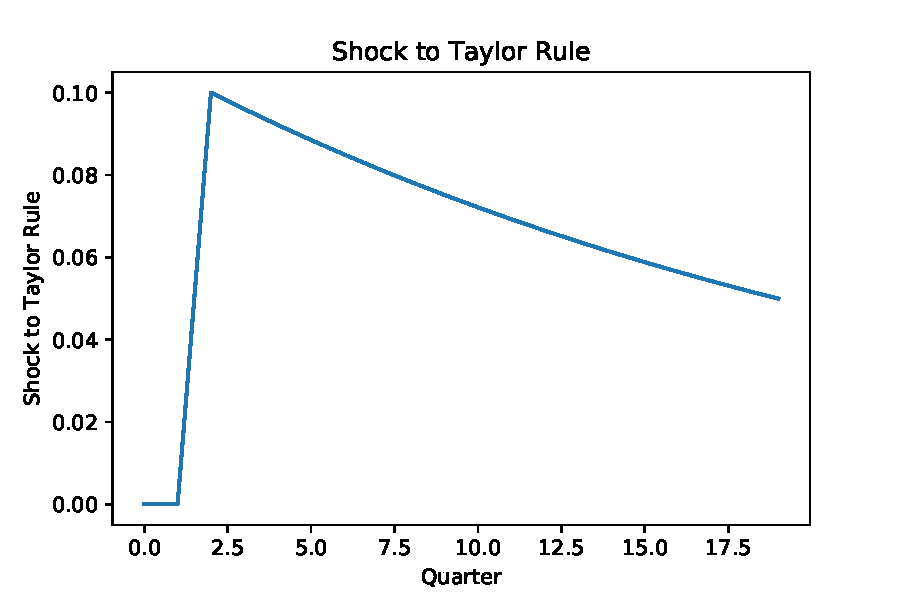
\includegraphics[width=0.45\textwidth]{../Code/Dolo/Figures/shock.pdf}
	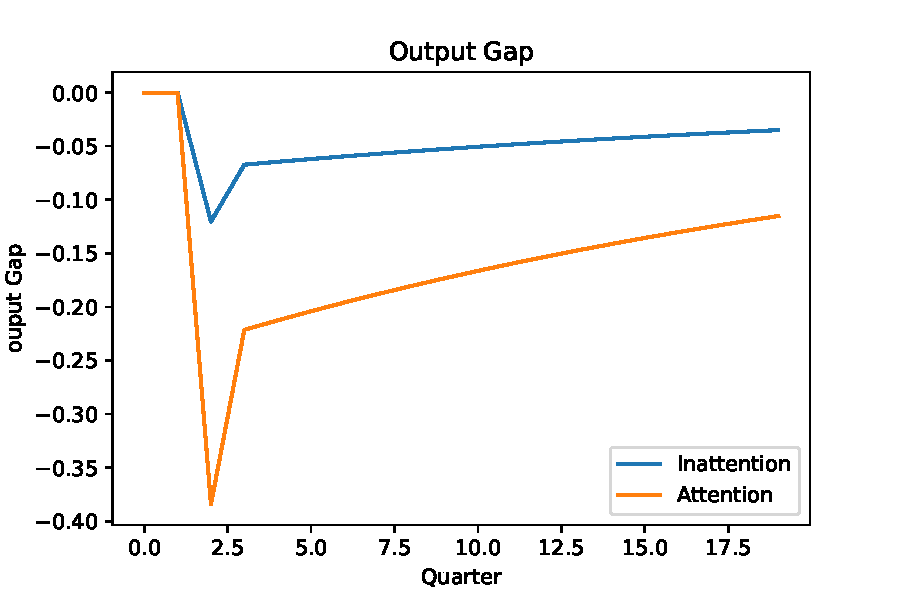
\includegraphics[width=0.45\textwidth]{../Code/Dolo/Figures/output_gap.pdf}
	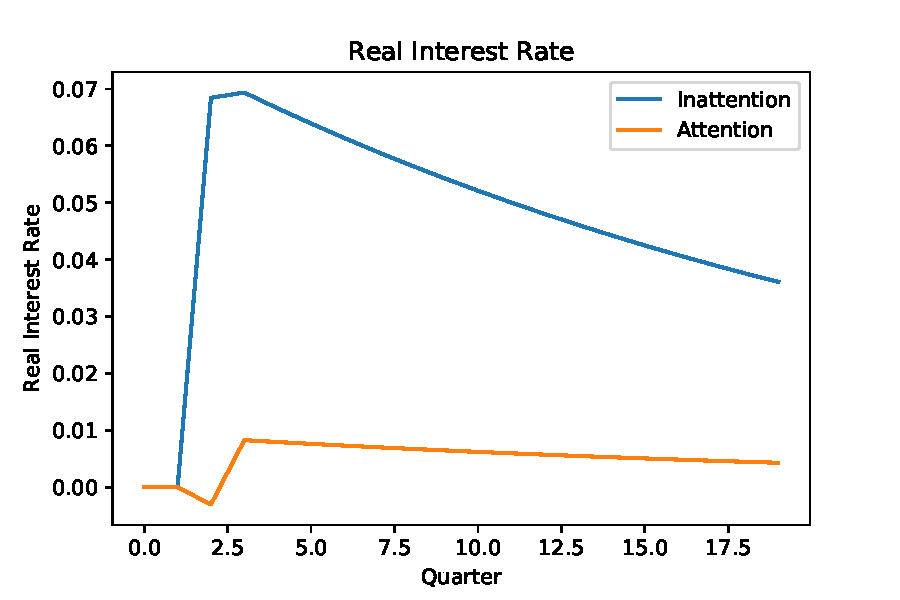
\includegraphics[width=0.45\textwidth]{../Code/Dolo/Figures/real_rate.pdf}
	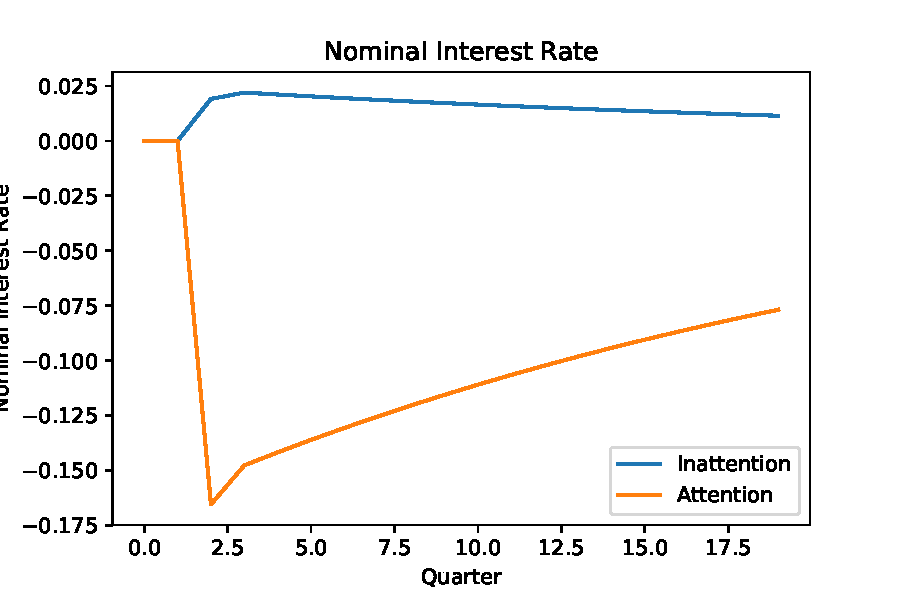
\includegraphics[width=0.45\textwidth]{../Code/Dolo/Figures/nominal_rate.pdf}
	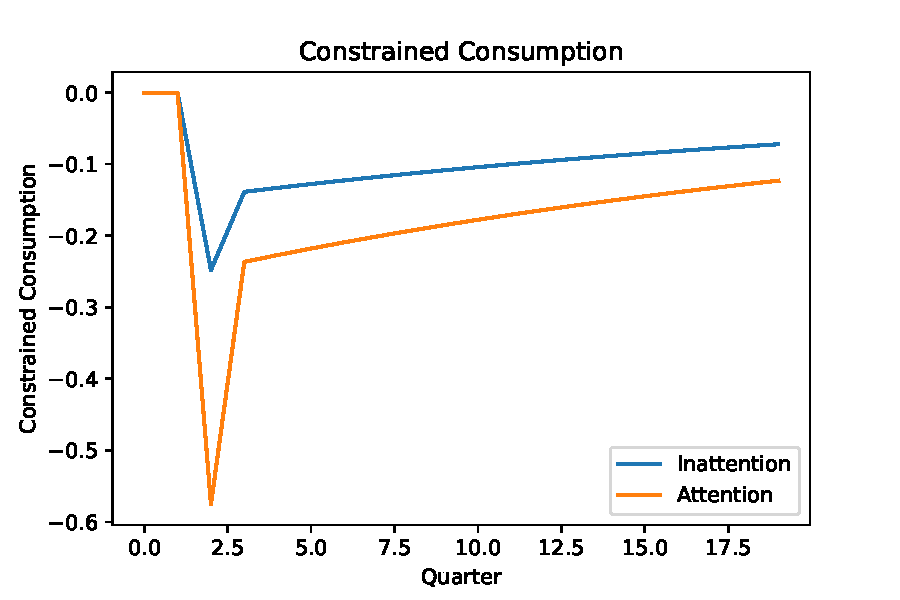
\includegraphics[width=0.45\textwidth]{../Code/Dolo/Figures/constrained.pdf}
	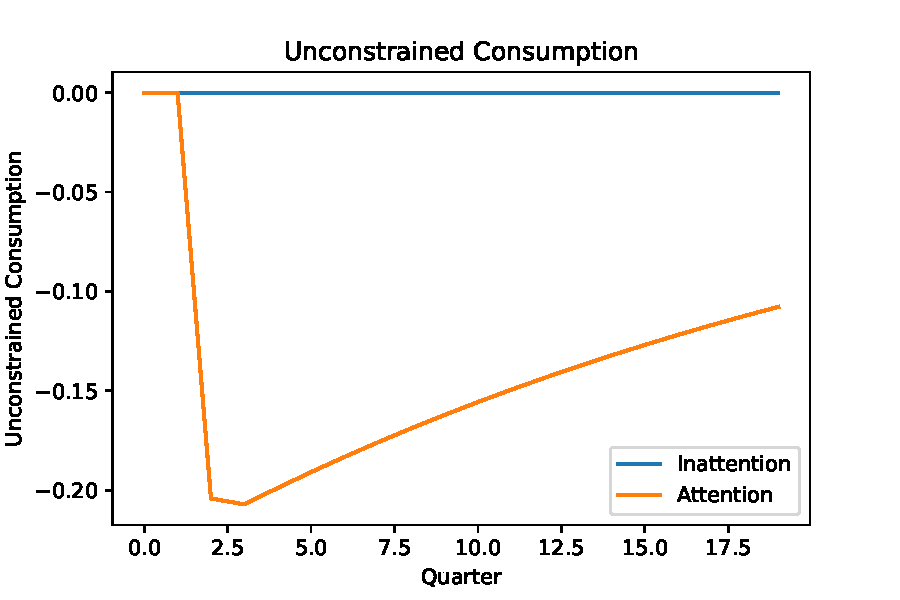
\includegraphics[width=0.45\textwidth]{../Code/Dolo/Figures/unconstrained.pdf}
	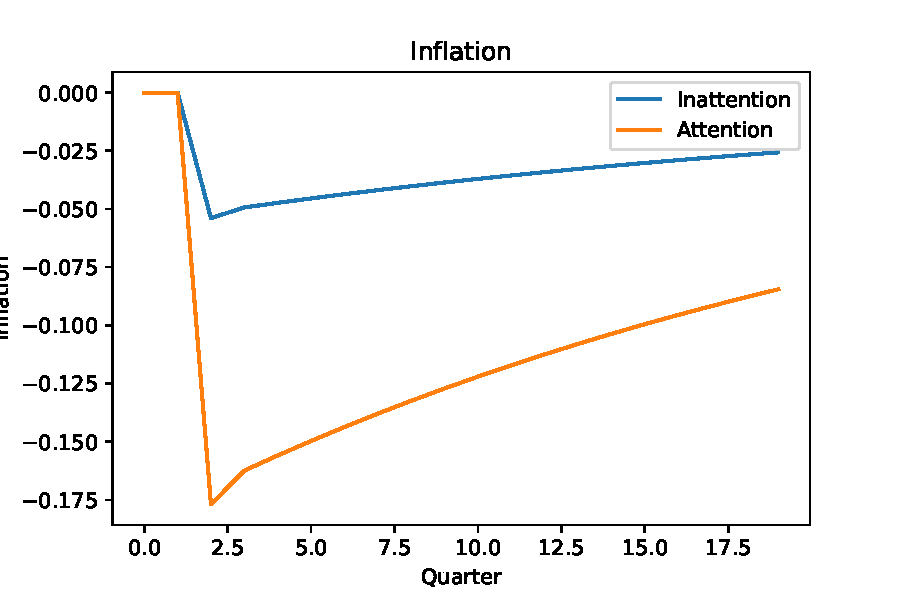
\includegraphics[width=0.45\textwidth]{../Code/Dolo/Figures/inflation.pdf}
	\caption{Impulse Response Functions to a Persistent Taylor Rule Shock}
	\label{fig:ImpulseResponse}
\end{figure}
\subsection{Forward Guidance Puzzle}
\begin{figure}
	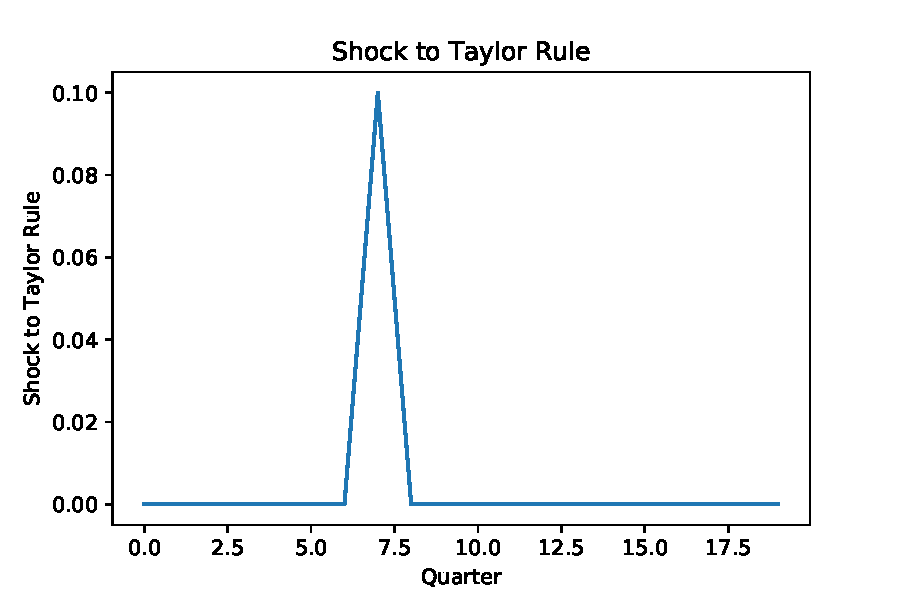
\includegraphics[width=0.45\textwidth]{../Code/Dolo/Figures/shock_fwd_guid.pdf}
	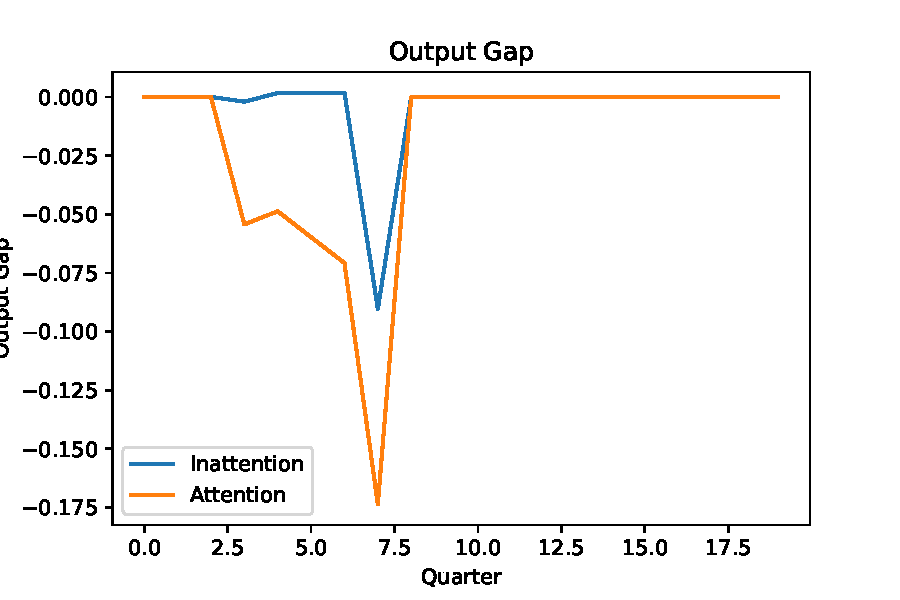
\includegraphics[width=0.45\textwidth]{../Code/Dolo/Figures/output_fwd_guid.pdf}
	\caption{Forward Guidance Puzzle}
	\label{fig:FwdGuidance}
\end{figure}



\section{A Simple Model with Adjustable Rate Mortgages}


\section{A Simple Model with Refinancing}

% Remove or comment out the next two lines if you are not using bibtex.
\bibliographystyle{aea}
\bibliography{WhoPaysAttention}

% The appendix command is issued once, prior to all appendices, if any.
\appendix

\end{document}

